\chapter{System DIMAC-EK}

Niniejsza praca magisterska związana jest bezpośrednio z systemem sterowania urządzeniami energetyki kolejowej. Niniejszy rozdział zawiera pobieżny opis systemu, by przybliżyć czytelnikowi tematykę pracy.

\section{Wstęp}

\subsection{Funkcje}

System DIMAC-EK jest złożonym rozwiązaniem zajmującym się sterowaniem automatyką kolejową.\cite{dimacek-katalog} Jego głównym zadaniem jest zapewnienie drożności tras kolejowych podczas trudnych warunków pogodowych oraz dostarczanie pomiarów związanych z tą czynnością. Czyności te dotyczą głównie okresu zimowego, gdy mróz oraz śnieg jest w stanie blokować działanie rozjadów kolejowych oraz tarasować przejazd. W skład systemu wchodzą nastepujące elementy:

\begin{itemize}
\item oświetlanie oraz osuszanie terenów kolejowych
\item ochrona antywłamaniowa i przeciwpożarowa
\item pomiar zużycia energii elektrycznej
\item elektryczne ogrzewanie rozjadu
\end{itemize}

\subsection{Budowa}
Rozwiązanie będące przedmiotem niniejszej pracy ma bezpośredni związek z ostatnią funkcją systemu - elektrycznym ogrzewaniem rozjazdów. Jest ono realizowane za pomocą grzałek elektrycznych montowanych na torach, które połączone są z urządzeniami nadzorującymi ich pracę. Urządzenia dzielą się na dwie grupy. Pierwszą z nich są sterowniki, które kontrolują  prace grzałek na podstawie odczytów z przetworników pogodowych. Druga to urządzenia nadrzędne, które służą do zdalnego sterowania wszystkimi sterownikami oraz zbierania i dalszego przesyłu ich danych. Dane te są arhiwizowane przez serwer, umożliwiając ich analizę.

Strukturę systemu przedstawia poniższy schemat:
\begin{figure}[h]
	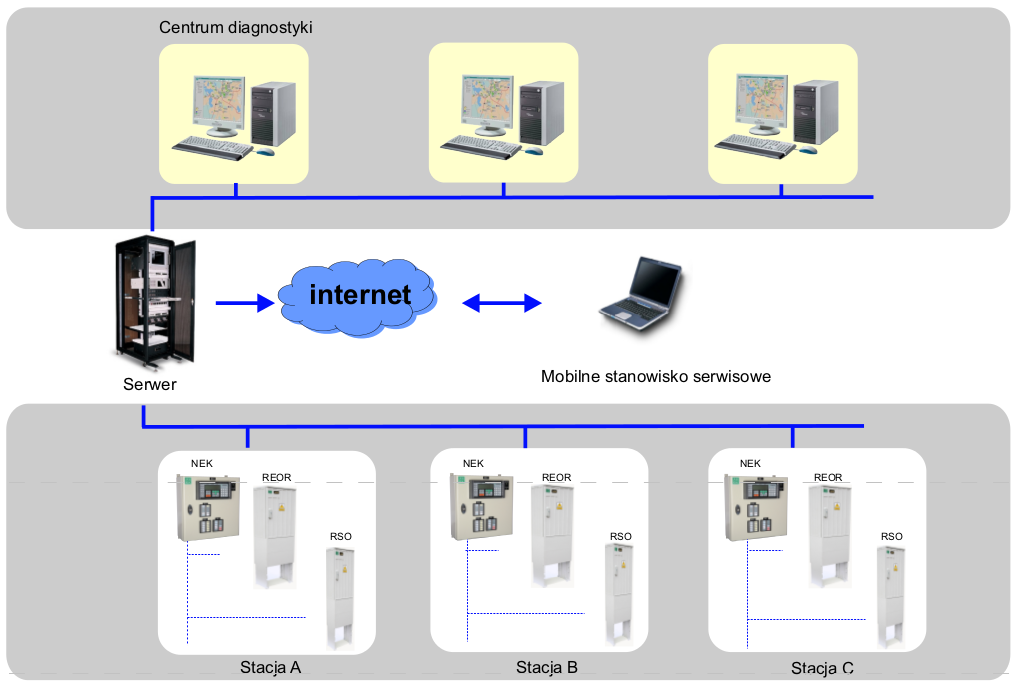
\includegraphics[height=85mm]{./img/dimacek_struktura.png}
	\caption{Struktura systemu DIMAC-EK}
	\label{fig:dimacek-scheme}
\end{figure}

\subsection{Standard otwarty}
DIMAC-EK został wdrożony przez firmę Arex na zamówienie Polskich Lini Kolejowych. Po odniesieniu sukcesu na kilku stacjach, system został wdrożony w całym kraju. W związku z tym nastąpiła koniecznośc utworzenia otwartego standardu, który jasno określa wymogi dla dostarczanych przez firmy urządzeń grzewczych. Standard ten został nazwany Standardem KHA. Każda firma produkująca sprzęt zgodny z KHA może być dostawcą urządzeń dla Polskich Kolei. Na kupno urządzeń oraz administrację systemem ogłaszane są okresowo przetargi.

\section{Struktura systemu}
System DIMAC-EK składa się z następujących warstw:\cite{dimacek-wytyczne}
\begin{itemize}
\item Warstwa urządzeń pomiarowych - przetworniki pogodowe
\item Warstwa urządzeń wykonawczych - grzałki elektryczne
\item Warstwa autotnomicznych rozdzielnic energetycznych - sterowniki RESO3F
\item Warstwa archiwizacji i obróbki danych - sterowniki nadrzędne NEK
\item Warstwa komunikacji systemu - sieć GPRS lub LAN
\item Warstwa nadzoru i zarządzania - stanowiska diagnostyczne + serwer
\end{itemize}


\subsection{Warstwa urządzeń pomiarowych}
Przetworniki zaopatrują sterowniki w dane pogodowe. Jeden sterownik może odbierać dane z wielu przetworników. Dostępne są następujące typy przetworników pogodowych:
\begin{itemize}
\item temperatury powietrza
\item prędkości wiatru
\item detekcji deszczu (czujnik wilgoci)
\item detekcji śniegu
\item temperatury szyny odniesienia (tzw. ,,zimnej'')
\item temperatury szyny ogrzewanej (tzw. ,,ciepłej'')
\item detekcji śniegu nawiewanego na rozjazd
\end{itemize}

\subsection{Warstwa urządzeń wykonawczych}
Grzejniki można podzielić ze względu na sposób i miejsce ich montażu na torach oraz na moc. Wszystkie parametry grzejników dopusczonych do użycia na torach znaleźć można w dokumentacji systemu dostarczanej przez PKP.

\subsection{Warstwa autonomicznych rozdzielnic energetycznych}
Rozdzielnice RESO przeznaczone są do sterowania obwodami elektrycznego ogrzewania rozjazdów oraz obwodami oświetleniowymi. Poza funkcją sterującą dokonują diagnostyki obwodów oraz przetworników pomiarowych. Rozdzielnice zawierają sterowniki oraz moduły sterująco-diagnostyczne, ktore sterują pracą grzałek. Sterowniki współpracują z urządzeniami nadrzędnym NEK, dzieki czemu pracę rozdzielnicy RESO można kontrolować z poziomu zdalnych stanowisk dyspozytorskich oraz stron www. Pozostałe elementy składowe rozdzielniczy widoczne są na zdjęciu zamieszczonym poniżej:

\begin{figure}[t]
	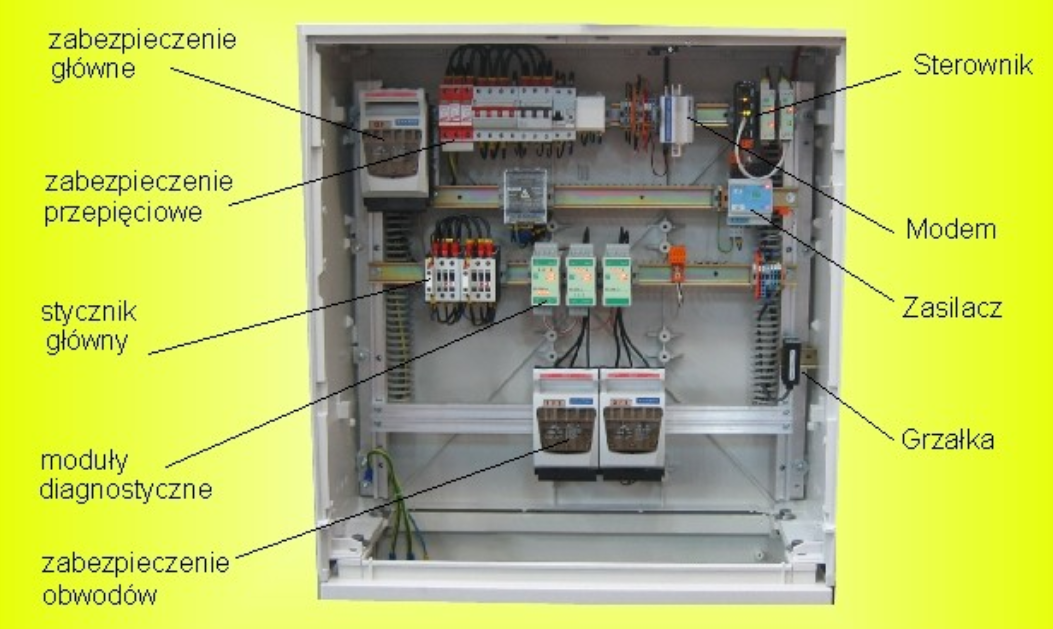
\includegraphics[height=95mm]{./img/dimacek_rozdzielnica.png}
	\caption{Budowa rozdzielnicy RESO}
	\label{fig:dimacek-reso}
\end{figure}

\subsection{Warstwa archiwizacji i obróbki danych}